% Contributions are much appreciated, in order to contribute to this project, head over to this repository:
% https://github.com/bshramin/uofa-eng-assignment

\documentclass[11pt,letterpaper]{article}
\textwidth 6.5in
\textheight 9.in
\oddsidemargin 0in
\headheight 0in
\usepackage{graphicx}
\usepackage{fancybox}
\usepackage[utf8]{inputenc}
\usepackage{epsfig,graphicx}
\usepackage{multicol,pst-plot}
\usepackage{pstricks}
\usepackage{amsmath}
\usepackage{amsfonts}
\usepackage{amssymb}
\usepackage{eucal}
\usepackage[left=2cm,right=2cm,top=2cm,bottom=2cm]{geometry}
\pagestyle{empty}
\DeclareMathOperator{\tr}{Tr}
\newcommand*{\op}[1]{\check{\mathbf#1}}
\newcommand{\bra}[1]{\langle #1 |}
\newcommand{\ket}[1]{| #1 \rangle}
\newcommand{\braket}[2]{\langle #1 | #2 \rangle}
\newcommand{\mean}[1]{\langle #1 \rangle}
\newcommand{\opvec}[1]{\check{\vec #1}}
\renewcommand{\sp}[1]{$${\begin{split}#1\end{split}}$$}

\usepackage{lipsum}

\usepackage{listings}
\usepackage{color}

\definecolor{codegreen}{rgb}{0,0.6,0}
\definecolor{codegray}{rgb}{0.5,0.5,0.5}
\definecolor{codepurple}{rgb}{0.58,0,0.82}
\definecolor{backcolour}{rgb}{0.95,0.95,0.92}

\lstdefinestyle{mystyle}{
	backgroundcolor=\color{backcolour},   
	commentstyle=\color{codegreen},
	keywordstyle=\color{magenta},
	numberstyle=\tiny\color{codegray},
	stringstyle=\color{codepurple},
	basicstyle=\footnotesize,
	breakatwhitespace=false,         
	breaklines=true,                 
	captionpos=b,                    
	keepspaces=true,                 
	numbers=left,                    
	numbersep=5pt,                  
	showspaces=false,                
	showstringspaces=false,
	showtabs=false,                  
	tabsize=2
}

\lstset{style=mystyle}

\begin{document}
\pagestyle{plain}

\begin{flushleft}
	Estudiante: Fabio Quimbay\\
	Email: fabio.quimbay883@comunidadunir.net\\
	Profesor: Miguel Ángel Cabeza\\
	Fecha: Noviembre 16 de 2022\\
\end{flushleft}

\begin{flushright}\vspace{-15mm}

\includegraphics[height=2cm]{logo.png}
\end{flushright}
 
\begin{center}\vspace{0cm}
\textbf{\large PER5786 2022-2023  Cálculo (GFI) - PER5786 2022-2023}\\
Actividad 1. Boletín de problemas
\end{center}

 
\rule{\linewidth}{0.1mm}
%%%%%%%%%%%%%%%%%%%%%%%%%%%%%%%%%%%%%%%%%%%%%%%%%%%%%%%%%%%%%%%%%%%%%%%%

\bigskip
\bigskip

%%%%%%%%%%%%%%%%%%%%
\textbf{Objetivos de la actividad}\\

A través de este boletín de ejercicios sencillos podrás practicar los conocimientos adquiridos en los temas que van del 1 al 3.\\

\textbf{Descripcipción de la actividad}\\

Resuelve los siguientes problemas rápidos de manera individual. Para ello, puedes usar cualquier herramienta informática que permita la redacción de expresiones matemáticas, pero te recomendamos que uses estándares electrónicos tales como HTML, Markdown, LaTeX o LyX. Además de subir el documento al campus, también puedes aportar un enlace público a un repositorio. 

%%%%%%%%%%%%%%%%%%%%

\begin{enumerate}

	%%%%%%%%%%%%%%%%%%%%
	\item Simplifica la siguiente expresión con potencias: $\frac{a^3b^4c^7}{a^{-2}b^5\sqrt{(c)}}$
	%%%%%%%%%%%%%%%%%%%%

	\textbf{Solución}: $\frac{a^5 \cdot c^{\frac{13}{2}}}{b}$

	%%%%%%%%%%%%%%%%%%%%
	\item Calcular el cociente de potencias: $\frac{2^33^2}{3^32}$
	%%%%%%%%%%%%%%%%%%%%

	\textbf{Solución}: $\frac{2^2}{3} = \frac{4}{3}$
	
	%%%%%%%%%%%%%%%%%%%%
	\item Calcular: $\left( \frac{\left( 2 \frac{3}{9} : 3\right)^{-1}}{\left(\frac{9}{4}\right)^2\left(\frac{2}{5}\right)^{-1}} \right)$
	%%%%%%%%%%%%%%%%%%%%

	\textbf{Solución}:
	\begin{align}
		\frac{\left( 2 \frac{3}{9} : 3\right)^{-1}}{\left(\frac{9}{4}\right)^2\left(\frac{2}{5}\right)^{-1}}
		= \frac{\left(  \frac{2}{9} \right)^{-1}}{\left(\frac{9}{4}\right)^2\left(\frac{2}{5}\right)^{-1}}
		= \frac{\left(  \frac{2}{5} \right)}{\left(\frac{9}{4}\right)^2\left(\frac{2}{9}\right)}
		= \frac{\left(  \frac{2}{5} \right)}{\left(\frac{9}{4}\right)^2\left(\frac{1}{2}\right)}
		= \frac{16}{45}
		= \frac{2^4}{3^25}
	\end{align}

	%%%%%%%%%%%%%%%%%%%%
	\item Calcular y: $\log_{2}y^3 = 6$
	%%%%%%%%%%%%%%%%%%%%

	\textbf{Solución}:
	\begin{align*}
		\log_{2}y^3 &= 6 \Rightarrow \\  
		2^6 &= y^3 \\
		\sqrt[3]{2^6} &= \sqrt[3]{y^3} \\
		y &= 2^{\frac{6}{3}} = 2^2 = 4
	\end{align*}
	
	%%%%%%%%%%%%%%%%%%%%
	\item Sea $\log_{10}2 = 0,3010$, calcula el siguiente logaritmo: $\log_{10}\sqrt[4]{8}$
	%%%%%%%%%%%%%%%%%%%%

	\textbf{Solución}:

	\begin{align*}
		&= \log_{10}\sqrt[4]{8} \Rightarrow \log_{10}\sqrt[4]{2^3} = \log_{10}2^{\frac{3}{4}} = \frac{3}{4}\log_{10}2 = \frac{3}{4} \cdot (0.3010) = 0.22575
	\end{align*}

	%%%%%%%%%%%%%%%%%%%% 	
	\item Convierte los siguientes ángulos de radiantes a grados sexagesimales: $3\;rad, 2\pi/5\;rad, 3\pi/20$. 
	%%%%%%%%%%%%%%%%%%%%

	\textbf{Solución}:
	
	\begin{align*}
		\boxed{ r = g \cdot \frac{\pi}{180}\,radianes} \quad \boxed{ g = r \cdot \frac{180}{\pi}\,grados}
	\end{align*}
	
	De tal forma que:
	
	\begin{align}
		a)\,3\,rad \Rightarrow g = 3 \cdot \frac{180}{\pi} grados = \frac{580}{\pi} = 171.887^{\circ}\\
		b)\,\frac{2 \cdot \pi}{5}\,rad \Rightarrow g = \frac{2 \cdot \pi}{5} \cdot \frac{180}{\pi} grados = 2 \cdot 36 = 72^{\circ}\\
		c)\,\frac{3 \cdot \pi}{20}\,rad \Rightarrow g = \frac{3 \cdot \pi}{20} \cdot \frac{180}{\pi} grados = 3 \cdot 9 = 27^{\circ}
	\end{align}
	
	%%%%%%%%%%%%%%%%%%%%
	\item Sabiendo que $cos\,\alpha=\frac{1}{4}$ y que el ángulo está en el primer cuadrante, calcular las restantes razones trigonométricas para dicho ángulo.
	%%%%%%%%%%%%%%%%%%%%

	\textbf{Solución}:
	
	Dada la ecuación $cos\,\alpha = \frac{1}{4}$ y de acuerdo al teorema de pitágoras para triángulos rectángulos $a^2 = b^2 + c^2$ en donde $\textbf{b}$ y $\textbf{c}$ 
	corresponden a los catetos y $\textbf{a}$ a la hipotenusa, podemos conocer que en la ecuación original el 1 corresponde al cateto $\textbf{a} = 3$ y la hipotenusa $\textbf{c} = 4$; 
	por lo que es fácilmente poder determinar el valor del otro cateto, a saber $\textbf{b} = 3$. \\
	
	De tal forma podemos expresar las razones trigonométricas como siguen:
	
	\begin{itemize}
		\item $cos\,\alpha = \frac{1}{4}$
		\item $sec\,\alpha = \frac{1}{cos\,\alpha} = \frac{1}{\frac{1}{4}} = 4$
		\item $sen\,\alpha = \frac{b}{a} = \frac{3}{4}$
		\item $tan\,\alpha = \frac{sen\,\alpha}{cos\,\alpha} = \frac{\frac{3}{4}}{\frac{1}{4}} = \frac{12}{4} = 3$
		\item $csc\,\alpha = \frac{1}{sen\,\alpha} = \frac{a}{b} = \frac{3}{4}$
		\item $cot\,\alpha = \frac{1}{tan\,\alpha} = \frac{cos\,\alpha}{sen\,\alpha} = \frac{c}{b} = \frac{1}{3}$
	\end{itemize}

	%%%%%%%%%%%%%%%%%%%%
	\item Calcula la altura de una torre de refrigeración de una central nuclear sabiendo que la sombra mide 271 metros cuando los rayos solaren forman un ángulo de $30^\circ$.
	%%%%%%%%%%%%%%%%%%%%

	\textbf{Solución}:

	Primero establecemos el valor de la hipotenusa (c) con base en la información existente del ángulo ($\alpha$) y el cateto adyacente ($b$) que equivale a la 
	longitud de la sombra con un valor de 271 metros, a saber:
	
	\begin{align}
		cos\,\alpha &= \frac{b}{c} \Rightarrow cos\,30^{\circ} = \frac{271}{c}\\
		\Rightarrow c &= \frac{271}{cos\,30^{\circ}} = \frac{271}{0.866025} = 312.924\,m
	\end{align}

	Al hallar la hipotenusa (c) y con los demás valores ya conocidos, podemos establecer la altura de la torre de refigeración, así:
	
	\begin{align}
		sin\,\alpha &= \frac{a}{c} \Rightarrow a = sin\,30^{\circ} \cdot c \\
		\Rightarrow a &= sin\,30^{\circ} \cdot 312.924 = 156.462\,m
	\end{align}

	A través del teorema de pitágoras podemos hacer una breve validación, así:

	\begin{align*}
		c^2 &= a^2 + b^2\\
		312.924^2 &= 156.462^2 + 271^2\\
		97921.4 &= 97921.4
	\end{align*}

	%%%%%%%%%%%%%%%%%%%%
	\item Calcula sin usar la calculadora ni tablas trigonométricas: $cos\;5\pi/12$, $cos\;7\pi/6$.
	%%%%%%%%%%%%%%%%%%%%

	\textbf{Solución}:
	
	Con base en la imagen a continuación podemos establecer las siguientes razones trigonométricas de ángulos y radianes, podemos determinar:
	
	\begin{center}
	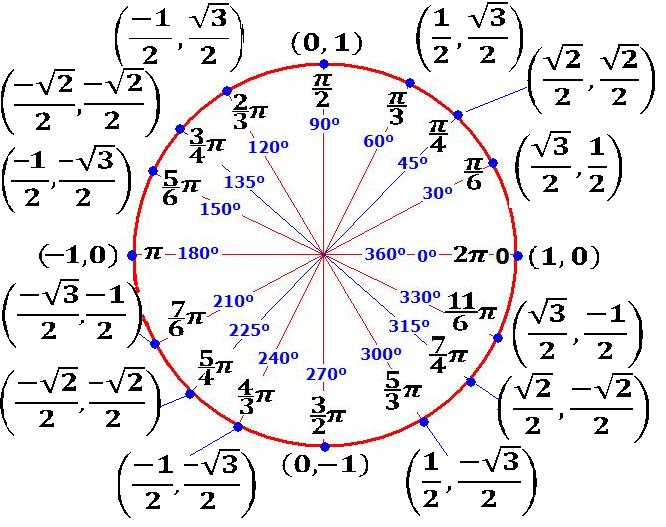
\includegraphics[height=4cm]{circulo.jpeg}
	\end{center}

	a) Lo primero es establecer una equivalencia del ángulo $\frac{5\pi}{12}$ a saber:
	
	\begin{align*}
		\frac{5\pi}{12} &= \frac{\pi}{6} + \frac{\pi}{4} = \frac{4\pi + 6\pi}{24} = \frac{10\pi}{24} 
	\end{align*}

	De tal forma, que podremos establecer la siguiente equivalencia:
	
	\begin{align*}
		cos\,\frac{5\pi}{12} &= cos\left(\frac{\pi}{6} + \frac{\pi}{4}\right) \Rightarrow \\
		&= cos\left(\frac{\pi}{6}\right) \cdot cos\left(\frac{\pi}{4}\right) - sin\left(\frac{\pi}{6}\right) \cdot sin\left(\frac{\pi}{4}\right)
	\end{align*}

	Al hacer la equivalencia de radianes a grados, de acuerdo a la imagen, obtenemos:
	
	\begin{align*}
		&= \frac{\sqrt{3}}{2} \cdot \frac{\sqrt{2}}{2} - \frac{\sqrt{1}}{2} \cdot \frac{\sqrt{2}}{2}\\
		&= \frac{\sqrt{3 \cdot \sqrt{2}}}{4} - \frac{\sqrt{1 \cdot \sqrt{2}}}{4}\\
		&= \frac{\sqrt{6}}{4} - \frac{\sqrt{2}}{4}\\
		cos\,\frac{5\pi}{12} &= \frac{\sqrt{6} - \sqrt{2}}{4}
	\end{align*}

	b) Al tratar de establecer una equivalencia del ángulo $cos \frac{7\pi}{6}$ podemos encontrar que existe un ángulo opuesto, el cual es
	$- cos \frac{\pi}{6}$, pero con un signo negativo, por lo que su equivalente es:
	
	\begin{align*}
		cos\,\frac{7\pi}{6} &= - cos \frac{\pi}{6} = - \frac{\sqrt{3}}{2}
	\end{align*}

	%%%%%%%%%%%%%%%%%%%%
	\item Calcular el seno, el coseno y la tangente de $105^\circ$ en función del ángulo $210^\circ$. 
	%%%%%%%%%%%%%%%%%%%%

	\textbf{Solución}:

	Para la realización de este ejercicio se utilizará los teoremas del seno, coseno y tangente del ángulo medio, a saber:
	
	\textbf{Cálculo del seno}:
	\begin{align*}
		sin\,\frac{210^{\circ}}{2} &= sin\,105^{\circ} = \sqrt{\frac{1 - cos\,210^{\circ}}{2}} = \sqrt{\frac{1 - (-\frac{\sqrt{3}}{2})}{2}} = \sqrt{\frac{2  + \frac{\sqrt{3}}{2})}{2}}\\
		sin\,105^{\circ} &= \sqrt{\frac{2  + \sqrt{3}}{4}} = \frac{\sqrt{2 + \sqrt{3}}}{2}
	\end{align*}
		
	\textbf{Cálculo del coseno}:
	\begin{align*}
		cos\,\frac{210^{\circ}}{2} &= cos\,105^{\circ} = -\sqrt{\frac{1 + cos\,210^{\circ}}{2}} = -\sqrt{\frac{(1-\frac{\sqrt{3}}{2}) \cdot 2}{2 \cdot 2}} = -\sqrt{\frac{2-\sqrt{3}}{4}}\\
		cos\,105^{\circ} &= -\frac{\sqrt{2-\sqrt{3}}}{\sqrt{4}} = -\frac{\sqrt{2-\sqrt{3}}}{2} 
	\end{align*}		

	\textbf{Cálculo de la tangente}:
	\begin{align*}
		tan\,\frac{210^{\circ}}{2} &= tan\,105^{\circ} = \frac{1-cos\,210^{\circ}}{sin\,210^{\circ}} = \frac{\left(1-(-\frac{\sqrt{3}}{2})\right) 
			\cdot (-\frac{2}{1})}{(-\frac{1}{2}) \cdot (-\frac{2}{1})} = -2-\sqrt{3}
	\end{align*}	

\end{enumerate}


\end{document}

